\begin{figure}[!htbp]
  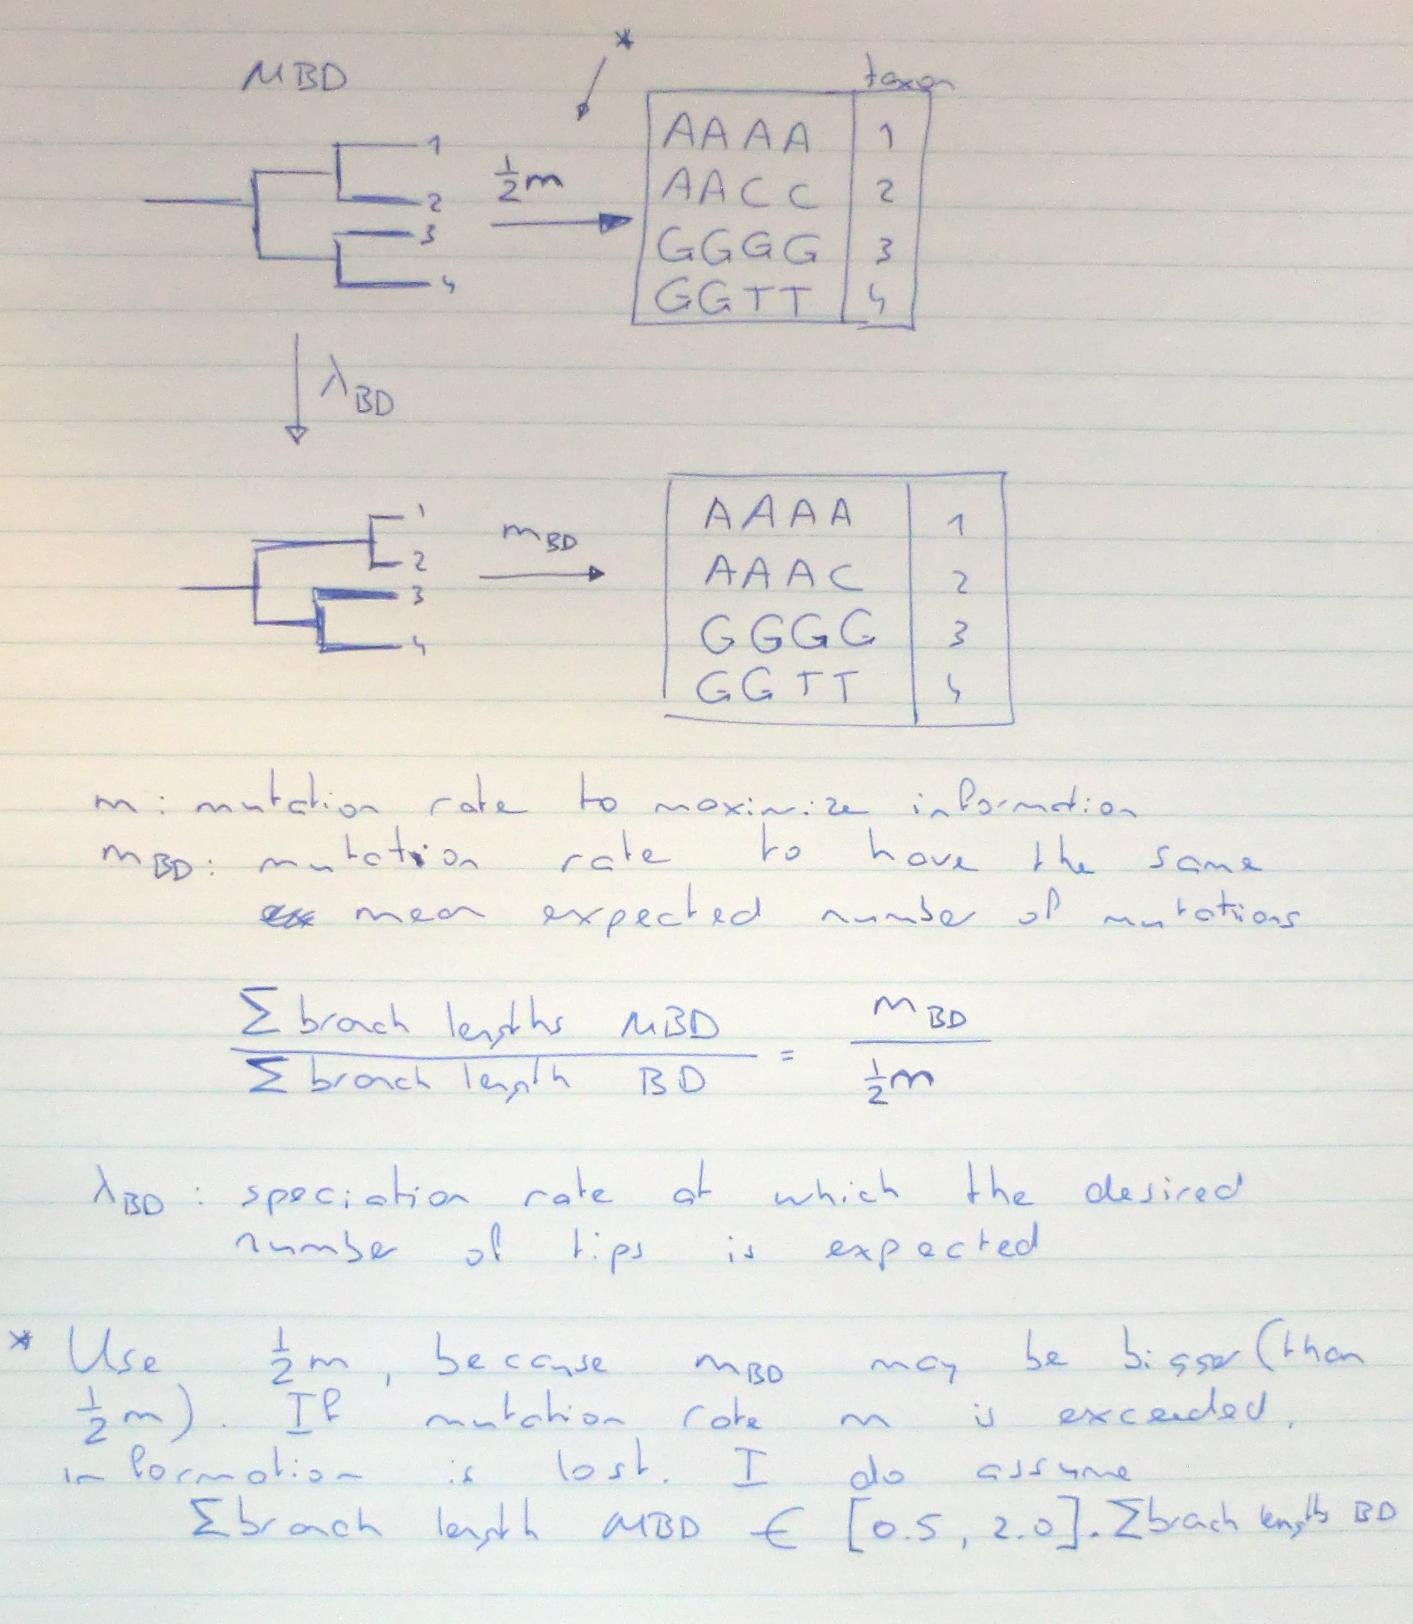
\includegraphics[width=\textwidth]{razzo-figures/fig_mbd.jpg}
  \caption{
    How to create twin trees and alignments. 
    From a focal MBD tree, a twin tree is produced as 
    such: (1) estimate the $\lambda_{BD}$ to get 
    the same expected number of tips, (2) simulate a BD tree 
    with that amount of tips (discard trees with different number of tips), 
    (3) estimate a mutation rate to get an alignment 
    with the same expected number of mutations, (4) simulate alignments 
    with that amount of mutations (discard those that don't, 
    the picture shows an alignment that should be discarded) 
  }
\end{figure}